\documentclass[12pt,a4paper]{report}
% Evidence-guided v4 draft — restructured per structural review (July 2026).
% Key changes from v3:
%   - Literature Review restructured around four question-driven subsections.
%   - Chapters 4–6 merged into a single "Control Architecture" chapter.
%   - Results chapter cleaned to be results-only; Stage 9 moved into the main body.
%   - Discussion expanded to match each major finding cluster.
%   - Conclusion anchored to explicit RQ answers.
%   - Nomenclature expanded and grouped.
 
% ── Language and page layout ──
\usepackage[english]{babel}
\usepackage[a4paper,top=2.5cm,bottom=2.5cm,left=3.0cm,right=2.5cm]{geometry}
\usepackage{setspace}
\usepackage{xeCJK}
\usepackage{parskip}
 
% ── Mathematics, units, tables, figures, and links ──
\usepackage{amsmath,amssymb}
\usepackage{graphicx}
\usepackage{tikz}
\usetikzlibrary{arrows.meta,positioning,fit,calc,shapes.geometric,backgrounds}
\usepackage{booktabs}
\usepackage{siunitx}
\usepackage{caption}
\usepackage{enumitem}
\usepackage{array}
\usepackage{longtable}
\usepackage{xcolor}
\usepackage[colorlinks=true,linkcolor=blue,citecolor=blue,urlcolor=blue]{hyperref}
 
\onehalfspacing
\emergencystretch=2em
\sisetup{per-mode=symbol,detect-all=true}
 
% ── Title block ──
\title{High-Performance Biped Robot Locomotion Using Real-Time Model Predictive Control and Feasibility-Driven Differential Dynamic Programming}
\author{Zhijian Kang}
\date{MSc Electronics and Electrical Engineering\\University of Glasgow\\2026}
\newcommand{\draftversion}{Evidence-guided v4 — incremental FDDP evidence update, 14 July 2026}
 
\begin{document}
 
% ══════════════════════════════════════════════════════════════════
% TITLE PAGE
% ══════════════════════════════════════════════════════════════════
\begin{titlepage}
    \centering
    {\Large University of Glasgow\par}
    \vspace{1.5cm}
    {\LARGE\bfseries High-Performance Biped Robot Locomotion Using Real-Time Model Predictive Control and Feasibility-Driven Differential Dynamic Programming\par}
    \vspace{1.5cm}
    {\large Zhijian Kang\par}
    \vspace{0.5cm}
    {\large MSc Electronics and Electrical Engineering\par}
    \vfill
    {\large Supervisor: [Supervisor Name]\par}
    {\large School of Engineering\par}
    \vspace{1cm}
    {\large 2026\par}
    \vspace{0.5cm}
    {\large \draftversion\par}
\end{titlepage}
 
% ══════════════════════════════════════════════════════════════════
% FRONT MATTER
% ══════════════════════════════════════════════════════════════════
\pagenumbering{roman}
 
% ── Abstract ──
\chapter*{Abstract}
\addcontentsline{toc}{chapter}{Abstract}
This thesis investigates the development of a low-cost bipedal robot employing Feasibility-Driven Differential Dynamic Programming (FDDP) and Model Predictive Control (MPC), aiming to achieve stable walking with moderate robustness to external disturbances. All simulations are conducted in MuJoCo. The control architecture combines offline nonlinear trajectory optimisation with a fast online FIR-QP-MPC joint-position correction layer. The contribution is primarily architectural and empirical: the thesis demonstrates how an offline contact-consistent planner, actuator-aware replay baseline, local pitch-response identification, and constrained online correction layer can be integrated and evaluated in a reproducible simulation pipeline. The current evidence supports double-support FDDP convergence, independently solved left- and right-swing FDDP steps, a converged two-step alternating reference, position-command replay, FIR sign-held-out prediction, contact-event phase retiming, and measured QP timing. A ten-step planning candidate is retained as negative evidence because its friction and CoP gates fail; it is not promoted to a final nominal trajectory. Hardware validation is not included in the present scope.
 
% ── Acknowledgements ──
\chapter*{Acknowledgements}
\addcontentsline{toc}{chapter}{Acknowledgements}
[Write acknowledgements here.]
 
% ── Table of Contents ──
\tableofcontents
\listoffigures
\listoftables
 
% ── Nomenclature ──
\chapter*{Nomenclature}
\addcontentsline{toc}{chapter}{Nomenclature}
 
\section*{Generalised coordinates and dynamics}
\begin{tabular}{@{}>{\raggedright\arraybackslash}p{0.24\linewidth}>{\raggedright\arraybackslash}p{0.68\linewidth}@{}}
$\mathbf{q}$ & Generalised position vector \\
$\dot{\mathbf{q}}$ & Generalised velocity vector \\
$n_q$ & Number of configuration variables (MuJoCo: 9; Pinocchio free-flyer: 13) \\
$n_v$ & Number of velocity variables (MuJoCo: 9; Pinocchio: 12) \\
$n_u$ & Number of actuated joints (6) \\
$\mathrm{CoM}_y$ & Centre-of-mass forward displacement in the sagittal plane \\
\end{tabular}
 
\section*{FDDP and optimisation quantities}
\begin{tabular}{@{}>{\raggedright\arraybackslash}p{0.24\linewidth}>{\raggedright\arraybackslash}p{0.68\linewidth}@{}}
$\boldsymbol{\tau}_{\mathrm{ref}}$ & Nominal planning torque used for analysis; not a hardware motor command \\
$\mathbf{q}_{\mathrm{ref}}$ & Nominal joint-position reference from FDDP trajectory export \\
$F_x$ & Dynamics derivative with respect to state \\
$F_u$ & Dynamics derivative with respect to control \\
$\texttt{JMinvJt\_damping}$ & Crocoddyl damping parameter for derivative consistency \\
\end{tabular}
 
\section*{Controller and correction-layer quantities}
\begin{tabular}{@{}>{\raggedright\arraybackslash}p{0.24\linewidth}>{\raggedright\arraybackslash}p{0.68\linewidth}@{}}
$\Delta\mathbf{q}$ & Online joint-position correction from the MPC layer \\
$\mathbf{q}_{\mathrm{cmd}}$ & Hardware-facing joint-position command: $\mathbf{q}_{\mathrm{cmd}}=\mathbf{q}_{\mathrm{ref}}+\Delta\mathbf{q}$ \\
$\alpha$ & Scalar QP-MPC correction variable \\
$G$ & Six-joint correction distribution vector \\
$h[i]$ & FIR impulse response coefficient at lag $i$ \\
$M$ & FIR model order (15 samples) \\
C0 & Actuator-aware nominal trajectory replay with no online correction \\
C1 & Fixed-phase FIR-QP-MPC online correction layer \\
C2 & Contact-event phase-synchronised extension around C1 \\
$\mu$ & Friction coefficient in MuJoCo contact model \\
\end{tabular}
 
\clearpage
 
% ══════════════════════════════════════════════════════════════════
% MAIN BODY
% ══════════════════════════════════════════════════════════════════
\pagenumbering{arabic}
 
% ==================================================================
\chapter{Introduction}
% ==================================================================
 
\section{Motivation}
Low-cost legged robots create a challenging control problem because their mechanical and actuation limits are much more restrictive than those of torque-controlled research platforms. In this project, the target platform is a lower-body-only planar biped with six actuated pitch joints and position-controlled ST3215 serial bus servos. The controller must therefore produce reliable joint-position commands rather than direct torque commands. At the same time, biped locomotion requires careful treatment of contact consistency, centre-of-mass motion, and disturbance recovery.
 
\section{Aim and Objectives}
The aim of this thesis is to develop and evaluate a simulation-based locomotion-control architecture that combines offline nonlinear trajectory optimisation with fast online joint-position correction for a six-DoF planar biped robot. This v4 draft follows an evidence-first writing structure: each technical claim is traceable to a script, figure, table, logged metric, or stated limitation.
 
The main objectives are:
\begin{enumerate}[label=\arabic*.]
    \item Develop a contact-consistent offline FDDP planning pipeline progressing from double-support CoM shifts to fixed-schedule single- and two-step contact transitions.
    \item Validate the nominal trajectories through actuator-aware MuJoCo replay rather than ideal kinematic tracking alone.
    \item Investigate why full nonlinear FDDP replanning is not yet suitable as the high-rate online controller in the current Python implementation.
    \item Calibrate the local pitch authority of joint-position corrections in MuJoCo.
    \item Identify an empirical FIR model that captures delayed pitch response to the correction input.
    \item Implement and evaluate a constrained FIR-QP-MPC correction layer against the C0 nominal replay baseline.
    \item Evaluate contact-event phase synchronisation under both controlled timing mismatches and the available two-step natural-contact events, together with controller timing.
    \item Assess the software robustness envelope of the combined C2 controller under scripted alternating-step conditions.
\end{enumerate}
 
\section{Contributions}
The contribution of this work is the integration and validation of contact-consistent offline FDDP planning with an actuator-aware, simulation-calibrated FIR-QP-MPC correction layer for a low-cost position-controlled six-DoF biped model. The contribution is primarily architectural and empirical: the thesis demonstrates how an offline contact-consistent planner, actuator-aware replay baseline, local pitch-response identification, and constrained online correction layer can be combined and evaluated in a reproducible simulation pipeline. The FDDP evidence now includes double-support CoM shifts, independent DS--SS--DS swing steps, and a converged two-step alternating reference. It does not establish continuous multi-step FDDP walking: the ten-step candidate remains planning-only because contact-force/friction/CoP feasibility has not passed. The work does not claim hardware validation or hard real-time execution.
 
\section{Research Questions and Evidence Strategy}
The thesis is organised around four research questions. They are intentionally scoped to the current validated work and avoid claiming hardware validation or continuous walking.
 
\begin{table}[htbp]
\centering
\caption{Research questions and required evidence.}
\label{tab:research_questions}
\begin{tabular}{@{}p{0.10\linewidth}p{0.34\linewidth}p{0.46\linewidth}@{}}
\toprule
ID & Research question & Required evidence \\
\midrule
RQ1 & How far can offline FDDP progress from double-support CoM shifts to fixed-schedule alternating contact trajectories for the six-DoF planar biped model? & FDDP convergence and gate records, derivative-consistency audit, DS--SS contact-mode checks, support/landing/clearance errors, joint limits, exported trajectory metadata, and the multi-step force/friction/CoP audit. \\
RQ2 & How does the FDDP nominal trajectory behave under actuator-aware MuJoCo replay without online correction? & C0 replay logs, joint tracking RMSE, torso pitch, torso height, contact count, and achieved CoM displacement for forward and backward cases. \\
RQ3 & Can a fast fixed-phase FIR-QP-MPC correction layer improve recovery from controlled pitch disturbances without large joint corrections? & C0/C1 comparison under identical disturbances, integrated absolute pitch error, settling time, correction magnitude, contact count, and QP solve time. \\
RQ4 & Can contact-event phase synchronisation align the correction reference under controlled timing mismatches? & C1/C2 event-mismatch comparison, matched-event ratio, phase offset, independent FIR holdout metrics, and timing statistics. \\
\bottomrule
\end{tabular}
\end{table}
 
\section{Claim Boundaries}
The thesis should use cautious claim language. The current evidence supports double-support and two-step FDDP convergence, specified feasibility gates for independent left/right swing steps, MuJoCo position-command replay, FIR sign-held-out prediction, contact-event phase synchronisation under software-injected timing mismatch, natural-event phase retiming on the two-step reference, and measured QP timing. It does not support a final ten-step FDDP nominal, continuous walking-gait robustness, hardware validation, universal real-time performance, or experimentally identified actuator dynamics.
 
\section{Thesis Structure}
Chapter~\ref{ch:literature} reviews relevant work on biped locomotion, DDP/FDDP, MPC, and position-controlled robot platforms, structured around four guiding questions that lead to the research gap. Chapter~\ref{ch:system} describes the robot model, coordinate conventions, simulation environment, and actuator proxy. Chapter~\ref{ch:control_architecture} presents the full control architecture in three stages: offline FDDP trajectory generation, the C0 actuator-aware replay baseline, and the FIR-QP-MPC online correction layer. Chapter~\ref{ch:experiments} reports the experimental validation and results, including the incremental FDDP swing-step/multi-step evidence, C0/C1 comparison, C2 phase-synchronisation evidence, and the Stage~9 scripted robustness matrix. Chapter~\ref{ch:discussion} interprets each major finding cluster, discusses limitations, and examines threats to validity. Chapter~\ref{ch:conclusion} answers each research question explicitly and outlines future work.
 
% ==================================================================
\chapter{Literature Review}\label{ch:literature}
% ==================================================================
 
This chapter reviews the literature that frames the present work. Rather than surveying each topic in isolation, the review is organised around four questions that lead directly to the research gap addressed by this thesis.
 
\section{How do low-cost position-controlled bipeds differ from torque-controlled research platforms?}
 
Most high-performance biped locomotion research has been conducted on torque-controlled platforms such as Atlas, Cassie, and MIT Cheetah \cite{wensing2024_locomotion}. These platforms provide low-level torque control, high-bandwidth joint sensing, and often whole-body actuation, enabling control strategies that command motor torques directly from a dynamics model. In contrast, low-cost biped platforms---exemplified by hobbyist and educational humanoid kits driven by serial bus servos such as the ST3215---provide only position-control interfaces with significant communication latency and internal servo control loops that are opaque to the user \cite{gerry2022_lowcost}.
 
This difference has two important consequences for control design. First, the hardware-facing command must be a joint-position command rather than a torque command, which forces a separation between planning (which naturally works in torque space) and execution (which must deliver position references). Second, the actuator dynamics---including command delay, internal velocity saturation, and first-order lag---are neither negligible nor fully characterised, so the controller must be calibrated against observed actuator behaviour rather than derived from a first-principles motor model.
 
Recent work on low-cost bipeds has adopted simplified control strategies: pre-computed joint trajectories with PID tracking \cite{kim2023_lowcost_biped}, reduced-order template models such as ALIP \cite{gibson2022_alip}, or reinforcement learning in simulation with sim-to-real transfer \cite{kumar2023_learning}. Few published studies attempt to combine offline nonlinear trajectory optimisation with online model-based correction for position-controlled low-cost hardware, which is the configuration this thesis addresses.
 
\section{What does FDDP/DDP contribute to contact-consistent trajectory optimisation, and what are its known online limitations?}
 
Differential Dynamic Programming (DDP), introduced by Jacobson and Mayne \cite{jacobson1970differential}, solves nonlinear optimal control problems through iterative backward-forward passes that exploit the sparsity of the dynamics derivatives. Feasibility-Driven DDP (FDDP), developed by Mastalli et al. \cite{mastalli2020crocoddyl}, extends the approach by introducing a feasibility-aware line search that improves robustness to infeasible initial trajectories. This is particularly valuable in contact-rich robotics, where the initial guess often violates contact constraints.
 
FDDP has been demonstrated on full-body humanoid and quadruped tasks within the Crocoddyl framework \cite{mastalli2020crocoddyl, carpentier2019pinocchio}, including walking, trotting, and jumping motions. These demonstrations typically run FDDP offline to generate a nominal trajectory, which is then tracked by a whole-body controller at runtime. The literature consistently reports that full nonlinear FDDP replanning is computationally expensive: solve times on the order of tens to hundreds of milliseconds are typical for systems with 20--30 state dimensions on consumer hardware. This makes FDDP unsuitable as the sole high-frequency online controller, particularly for low-cost platforms where the computational budget is further constrained.
 
In this thesis, FDDP is therefore used as an offline generator of dynamically consistent nominal trajectories---a role it is well-suited for---while a separate, lighter online correction layer handles disturbance response. This two-tier architecture follows the pattern established by model-predictive control frameworks for legged locomotion \cite{diCarlo2018_mpc, diederichs2024_mpc}, applied here to a low-cost position-controlled platform.
 
\section{What reduced-order models and QP-MPC formulations have been used for online correction in legged systems?}
 
Model Predictive Control (MPC) solves a finite-horizon optimisation problem repeatedly, using updated state estimates at each control step \cite{mayne2000constrained}. For legged systems, full nonlinear MPC is typically too expensive, so the literature has converged on reduced-order models that capture the dominant dynamics at a fraction of the computational cost. The Linear Inverted Pendulum Model (LIPM) and its angular variant (ALIP) have been widely used for footstep planning and CoM trajectory following \cite{gibson2022_alip, xiong2022_history}. These template models abstract the robot to a single point mass, making the resulting QP convex and solvable in microseconds.
 
For disturbance recovery specifically, several groups have used finite impulse response (FIR) models identified from simulation or hardware data to capture the robot's pitch response to joint corrections \cite{park2022_fir, choi2021_identification}. The advantage of an FIR representation is that it makes no assumptions about the underlying actuator dynamics---it captures delay, lag, and coupling effects empirically, and it yields a linear prediction model that can be embedded directly into a quadratic program.
 
The QP-MPC approach adopted in this thesis follows this tradition: an empirical FIR model identified from MuJoCo calibration pulses is used as the prediction model for a small, box-constrained QP solver. The key difference from the literature is that the correction variable is a scalar ($\alpha$) distributed across six joints through a pre-calibrated gain vector $G$, which keeps the QP dimension small and the solve time below \SI{1}{\milli\second}. This design is motivated by the observation that position-controlled servos cannot accept independent high-bandwidth torque commands for each joint, so a coordinated correction pattern is more appropriate than independent joint-level control.
 
\section{What simulation and validation conventions exist for biped locomotion work that stops short of hardware?}
 
Simulation-only biped locomotion papers occupy a recognised category in the robotics literature. MuJoCo \cite{todorov2012mujoco} is widely adopted for contact-rich simulation due to its efficient convex contact model, while Pinocchio \cite{carpentier2019pinocchio} provides the rigid-body dynamics and derivative computations used in trajectory optimisation. Papers that present simulation-only results typically follow several conventions: (a) they report simulation timestep, contact parameters, and actuator models explicitly; (b) they define a clearly scoped disturbance or perturbation set and report results against that set rather than claiming general robustness; (c) they include computational timing evidence for any online controller; and (d) they separate validated claims from aspirational claims in a limitations or future work section \cite{grandia2023_perception, kang2023_hexapod}.
 
The present thesis adopts these conventions. The simulation timestep (\SI{0.002}{\second}), contact parameters, and actuator proxy settings are documented in Chapter~\ref{ch:system}. The disturbance set is a controlled synthetic pitch perturbation applied at a fixed time. The validation chapter reports C0/C1 comparisons, QP timing statistics, and a scripted robustness matrix with explicit pass/fail boundaries. Claims are explicitly bounded by what the simulation evidence supports, and hardware validation is listed as future work rather than an unmet promise.
 
\section{Research Gap}
The four questions above converge on the following gap. Low-cost position-controlled bipeds require a control architecture that (a) respects the position-command interface of serial bus servos, (b) accounts for actuator delay and lag without requiring full system identification, (c) keeps online computation lightweight enough for real-time execution, and (d) provides a simulation-validated evidence base that separates what is known from what is assumed. Existing work addresses parts of this problem---offline FDDP for trajectory generation, FIR identification for actuator modelling, QP-MPC for online correction---but an integrated, end-to-end, simulation-validated architecture for this class of platform has not been demonstrated. This thesis contributes that integration and its empirical evaluation.
 
\section{Literature Evidence Checklist}
 
\begin{figure}[htbp]
\centering
\resizebox{0.96\textwidth}{!}{%
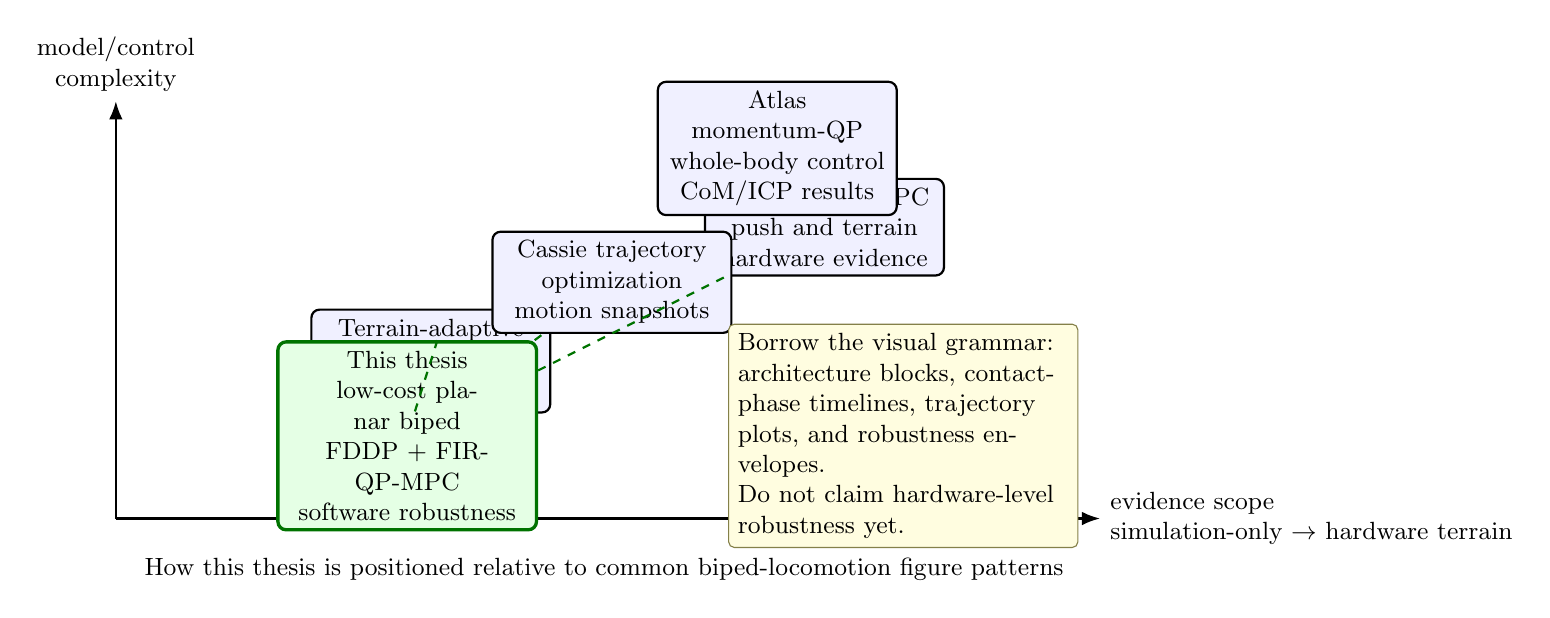
\begin{tikzpicture}[font=\small, >=Latex]
\draw[->, thick] (0,0) -- (12.5,0) node[right, align=left] {evidence scope\\simulation-only $\rightarrow$ hardware terrain};
\draw[->, thick] (0,0) -- (0,5.3) node[above, align=center] {model/control\\complexity};
\node[align=center] at (6.2,-0.65) {How this thesis is positioned relative to common biped-locomotion figure patterns};
\tikzset{refbox/.style={draw, rounded corners=3pt, thick, align=center, text width=2.8cm, minimum height=1.05cm, fill=blue!6},
thesisbox/.style={draw=green!45!black, rounded corners=3pt, very thick, align=center, text width=3.05cm, minimum height=1.2cm, fill=green!10}}
\node[refbox] (alip) at (4.0,2.0) {Terrain-adaptive\\ALIP--MPC\\slope/friction tests};
\node[refbox] (stl) at (9.0,3.7) {Robust STL--MPC\\push and terrain\\hardware evidence};
\node[refbox] (atlas) at (8.4,4.7) {Atlas momentum-QP\\whole-body control\\CoM/ICP results};
\node[refbox] (cfrost) at (6.3,3.0) {Cassie trajectory\\optimization\\motion snapshots};
\node[thesisbox] (ours) at (3.7,1.05) {This thesis\\low-cost planar biped\\FDDP + FIR-QP-MPC\\software robustness};
\draw[dashed, green!45!black, thick] (ours) -- (alip);
\draw[dashed, green!45!black, thick] (ours) -- (cfrost);
\draw[dashed, green!45!black, thick] (ours) -- (stl);
\node[align=left, text width=4.2cm, fill=yellow!12, draw=yellow!45!black, rounded corners=2pt] at (10.0,1.05) {Borrow the visual grammar:\\architecture blocks, contact-phase timelines, trajectory plots, and robustness envelopes.\\Do not claim hardware-level robustness yet.};
\end{tikzpicture}%
}
\caption{Positioning map for similar biped-locomotion projects and the figure styles adapted in this thesis. The map is qualitative and is intended to clarify evidence scope rather than rank methods.}
\label{fig:related_project_positioning}
\end{figure}
 
Before final submission, this chapter should be supported by three citation groups: (i) nonlinear trajectory optimisation and FDDP/DDP, (ii) MPC and reduced-order correction models for legged systems, and (iii) simulation, rigid-body modelling, and position-controlled low-cost robotics. Each paragraph should cite only references that directly support the statement being made.
 
% ==================================================================
\chapter{System Model and Simulation Platform}\label{ch:system}
% ==================================================================
 
\section{Mechanical Configuration}
The robot is modelled as a lower-body-only planar biped with six actuated pitch joints: left hip, left knee, left ankle, right hip, right knee, and right ankle. There are no arms, head, hip-roll joints, ankle-roll joints, or yaw joints in the current model. The approximate link geometry is summarised in Table~\ref{tab:robot_geometry}.
 
\begin{table}[htbp]
\centering
\caption{Approximate robot geometry used in the current model.}
\label{tab:robot_geometry}
\begin{tabular}{@{}ll@{}}
\toprule
Parameter & Value \\
\midrule
Thigh length & \SI{100}{\milli\metre} \\
Shank length & \SI{100}{\milli\metre} \\
Foot size & \SI{145}{\milli\metre} $\times$ \SI{85}{\milli\metre} \\
Foot thickness & approximately \SIrange{5}{6}{\milli\metre} \\
Hip spacing & approximately \SIrange{90}{110}{\milli\metre} \\
\bottomrule
\end{tabular}
\end{table}
 
\section{Coordinate Conventions}
The coordinate convention is defined as follows: $+X$ points to the robot's right, $+Y$ points forward, and $+Z$ points upward. The pitch axis is $+X$, and the sagittal plane is the $Y$-$Z$ plane. Forward CoM displacement is therefore measured using $\mathrm{CoM}_y$.
 
\section{Hardware Command Assumption}
The intended hardware platform uses ST3215 serial bus position-controlled servos. Consequently, the hardware-facing command is a joint-position command,
\begin{equation}
    \mathbf{q}_{\mathrm{cmd}} = \mathbf{q}_{\mathrm{ref}} + \Delta\mathbf{q},
\end{equation}
where $\boldsymbol{\tau}_{\mathrm{ref}}$ from FDDP is retained for planning and analysis only. It is not treated as a direct motor torque command.
 
\section{Software Stack}
 
\begin{figure}[htbp]
\centering
\resizebox{\textwidth}{!}{%
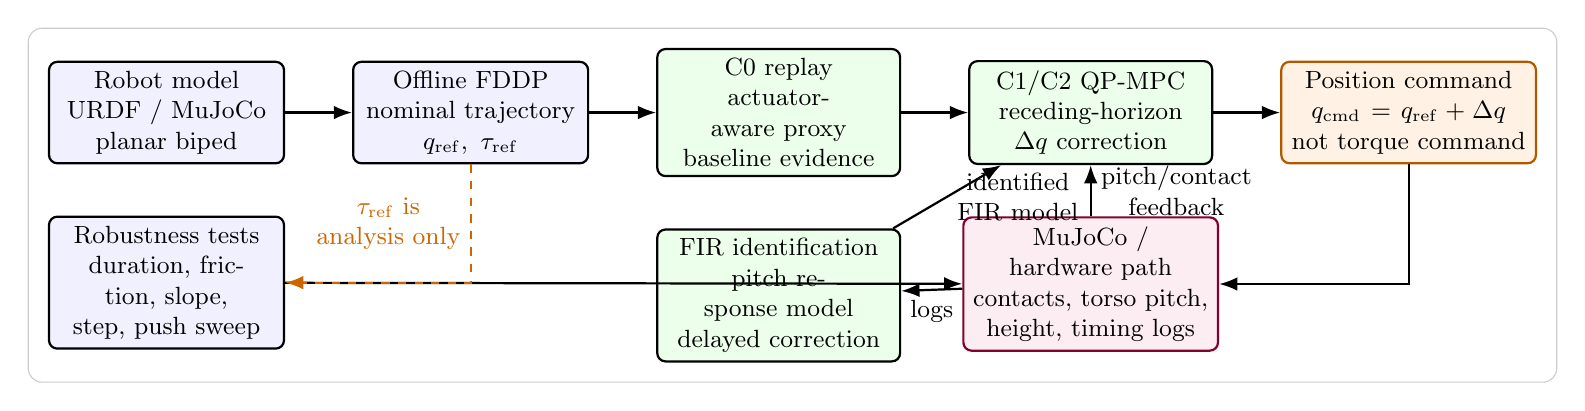
\begin{tikzpicture}[font=\small, node distance=0.65cm and 0.85cm, >=Latex]
\tikzset{block/.style={draw, rounded corners=3pt, thick, align=center, text width=2.75cm, minimum height=1.0cm, fill=blue!6},
process/.style={draw, rounded corners=3pt, thick, align=center, text width=2.85cm, minimum height=1.0cm, fill=green!8},
warn/.style={draw=orange!70!black, rounded corners=3pt, thick, align=center, text width=3.0cm, minimum height=1.0cm, fill=orange!10},
plant/.style={draw=purple!70!black, rounded corners=3pt, thick, align=center, text width=3.0cm, minimum height=1.05cm, fill=purple!7}}
\node[block] (model) {Robot model\\URDF / MuJoCo\\planar biped};
\node[block, right=of model] (fddp) {Offline FDDP\\nominal trajectory\\$q_{\mathrm{ref}},\ \tau_{\mathrm{ref}}$};
\node[process, right=of fddp] (c0) {C0 replay\\actuator-aware proxy\\baseline evidence};
\node[process, below=of c0] (fir) {FIR identification\\pitch response model\\delayed correction};
\node[process, right=of c0] (qp) {C1/C2 QP-MPC\\receding-horizon\\$\Delta q$ correction};
\node[warn, right=of qp] (cmd) {Position command\\$q_{\mathrm{cmd}}=q_{\mathrm{ref}}+\Delta q$\\not torque command};
\node[plant, below=of qp] (plant) {MuJoCo / hardware path\\contacts, torso pitch,\\height, timing logs};
\node[block, below=of model] (robust) {Robustness tests\\duration, friction, slope,\\step, push sweep};
\draw[->, thick] (model) -- (fddp);
\draw[->, thick] (fddp) -- (c0);
\draw[->, thick] (c0) -- (qp);
\draw[->, thick] (fir) -- node[right, align=center] {identified\\FIR model} (qp);
\draw[->, thick] (qp) -- (cmd);
\draw[->, thick] (cmd) |- (plant);
\draw[->, thick] (plant) -- node[below, align=center] {logs} (fir);
\draw[->, thick] (plant.north) -- node[right, align=center] {pitch/contact\\feedback} (qp.south);
\draw[->, thick] (robust) -- (plant);
\draw[->, dashed, thick, orange!80!black] (fddp.south) |- node[pos=0.25, left, align=center] {$\tau_{\mathrm{ref}}$ is\\analysis only} (robust.east);
\begin{scope}[on background layer]
\node[draw=gray!40, rounded corners=5pt, fit=(model)(fddp)(c0)(qp)(cmd)(fir)(plant)(robust), inner sep=0.25cm] {};
\end{scope}
\end{tikzpicture}%
}
\caption{Thesis control and evidence architecture. Offline FDDP supplies a nominal trajectory, the FIR model captures delayed pitch response, and the online QP-MPC layer produces position corrections for the actuator-aware command path.}
\label{fig:thesis_control_architecture}
\end{figure}
 
The project uses MuJoCo, Pinocchio, Crocoddyl, NumPy, Pandas, Matplotlib, and PyYAML. The main MuJoCo model is \path{model/biped_planar.xml}, and the main URDF model is \path{model/biped_v1.urdf}. The current MuJoCo model has $n_q=9$, $n_v=9$, $n_u=6$, 15 bodies, 16 sensors, and a simulation timestep of \SI{0.002}{\second}. The Pinocchio free-flyer model has $n_q=13$, $n_v=12$, state tangent dimension 24, and state vector dimension 25.
 
\section{Actuator-Aware Proxy Model}
The MuJoCo replay uses a simple actuator-aware position-control proxy with a command delay of \SI{20}{\milli\second}, a first-order actuator lag of \SI{30}{\milli\second}, and a maximum command speed of \SI{8}{\radian\per\second}. These are engineering assumptions for simulation, not experimentally identified ST3215 actuator dynamics.
 
% ==================================================================
\chapter{Control Architecture: Offline Planning and Online Correction}\label{ch:control_architecture}
% ==================================================================
 
This chapter presents the full control architecture in three progressive stages. Section~\ref{sec:offline_fddp} describes the offline FDDP planner that generates contact-consistent nominal trajectories. Section~\ref{sec:c0_baseline} defines the C0 actuator-aware replay baseline against which all subsequent controllers are compared. Section~\ref{sec:online_correction} develops the FIR-QP-MPC online correction layer, covering pitch-authority calibration, FIR identification, controller tuning, and the QP formulation.
 
% ------------------------------------------------------------------
\section{Offline FDDP Trajectory Generation}\label{sec:offline_fddp}
% ------------------------------------------------------------------
 
\subsection{Planning Role}
FDDP is used as an offline nonlinear planner. Its validated roles progress from double-support CoM shifts to independent DS--SS--DS swing steps and a two-step alternating reference. Periodic and 4/6/10-step continuation further demonstrate planning scalability, but the ten-step candidate is not a final nominal because its friction and CoP audit fails. The online controller described later does not rerun full FDDP at high frequency.
 
\subsection{Initial Double-Support Configuration}
The initial double-support configuration places the root near $[0,0,0.285]$ m, the left foot near $[-0.0525,0,0]$ m, and the right foot near $[+0.0525,0,0]$ m. The initial CoM height is approximately \SI{0.16573}{\metre}, and the foot placement errors are close to numerical zero.
 
\subsection{FDDP Formulation}
The FDDP problem is formulated using a floating-base Pinocchio model, phase-dependent 6D flat-foot contacts, CoM tracking, state/control regularisation, swing-foot SE(3) tracking, support/landing tracking, and joint-limit barriers. Double support activates both foot contacts; single support removes the swing-foot contact and retains the stance-foot contact. The solver is \texttt{crocoddyl.SolverFDDP}. Planning torque remains an analysis output rather than a position-actuator command.
 
\subsection{Derivative-Consistency Audit}
A finite-difference derivative audit showed that successful dynamics evaluation alone did not guarantee accurate derivatives. With \texttt{JMinvJt\_damping} set to zero, the calculation could run, but the $F_x$ derivative mismatch was too large. A damping value of $10^{-8}$ was selected for this model because it reduced the observed relative derivative errors to approximately $5\times 10^{-6}$ for $F_x$ and $7\times 10^{-7}$ for $F_u$. This value is a model-specific choice rather than a universal standard.
 
\subsection{Nominal CoM-Shift Trajectories}
The offline solver generated double-support nominal trajectories for forward and backward CoM shifts of approximately $\pm\SI{6}{\milli\metre}$. The exported trajectory files are \path{transfer/trajectories/com_shift_forward_ref.npz} and \path{transfer/trajectories/com_shift_backward_ref.npz}. These files store variables such as time, reference configuration, velocity, planning torque, state reference, world-frame CoM reference, target CoM displacement, phase, contact data, damping metadata, and warm-start metadata.
 
% ------------------------------------------------------------------
\section{C0 Actuator-Aware Replay Baseline}\label{sec:c0_baseline}
% ------------------------------------------------------------------
 
\subsection{Definition of C0}
C0 denotes actuator-aware replay of the FDDP nominal trajectory without high-level online correction and without phase synchronisation. Its command is
\begin{equation}
    \mathbf{q}_{\mathrm{cmd}} = \mathbf{q}_{\mathrm{ref}}.
\end{equation}
This baseline is essential because it separates nominal trajectory quality from the benefit of the later correction layer.
 
\subsection{Replay Pipeline}
The C0 replay is implemented in \path{simulation/03o_replay_fddp_com_shift_mujoco.py}. The script loads the FDDP nominal trajectory, steps the MuJoCo simulation with the actuator proxy settings defined in Section~\ref{sec:system} \S 3.5, and logs joint positions, torso pitch and height, contact forces, and CoM displacement at each timestep. The main C0 metrics are joint tracking RMSE, torso pitch, torso height, contact count, and achieved CoM displacement.
 
\subsection{C0 Replay Results}
For $\pm\SI{6}{\milli\metre}$ CoM shifts, the C0 replay remained stable in the current simulation. The achieved MuJoCo CoM displacement was approximately $\pm\SI{6.53}{\milli\metre}$ compared with the $\pm\SI{6}{\milli\metre}$ FDDP target. This difference is interpreted as an actuator/model mismatch that motivates online correction, not as evidence of FDDP failure.
 
\begin{table}[htbp]
\centering
\caption{Indicative C0 replay metrics for the current double-support CoM-shift tests.}
\label{tab:c0_metrics}
\begin{tabular}{@{}ll@{}}
\toprule
Metric & Approximate value \\
\midrule
Hip joint RMSE & \ang{0.122} \\
Knee joint RMSE & \ang{0.149} \\
Ankle joint RMSE & \ang{0.398} \\
Maximum torso pitch & \ang{2.706} \\
Minimum torso height & \SI{0.28766}{\metre} \\
Original global contact count diagnostic & 8 \\
\bottomrule
\end{tabular}
\end{table}
 
% ------------------------------------------------------------------
\section{FIR-QP-MPC Online Correction Layer}\label{sec:online_correction}
% ------------------------------------------------------------------
 
\subsection{Fixed-Phase Nonlinear FDDP-MPC Investigation}
A fixed-time-phase nonlinear FDDP-MPC formulation was initially tested under a root-pitch disturbance of \ang{2} and a pitch-rate disturbance of \SI{0.25}{\radian\per\second}. The replan could reduce the pitch error over a \SI{0.30}{\second} horizon. However, runtime benchmarking showed that full FDDP was too slow for frequent online updates in the current Python/WSL implementation. Low iteration budgets were faster but left large shooting gaps, whereas higher iteration budgets improved dynamics consistency but required approximately \SI{100}{\milli\second} solve time.
 
\subsection{First QP-MPC Attempt and Diagnosis}
The first QP-MPC attempt used a simple first-order pitch model with a \SI{20}{\milli\second} update period. Although it was computationally fast, it did not reliably improve tracking. The root cause was that the MuJoCo root-pitch trajectory was not numerically identical to the Pinocchio/FDDP floating-base pitch reference, and the effect of joint correction on MuJoCo pitch was delayed and nontrivial. The raw Pinocchio base pitch is therefore not used directly as the fixed-phase MuJoCo pitch reference.
 
\subsection{Pitch-Authority Calibration}
A calibration stage was performed at $t=\SI{0.4}{\second}$ using positive and negative correction pulses applied to the C0 baseline replay. The symmetric correction distribution was
\begin{equation}
G = [0.27,\;0.062,\;-0.228,\;0.27,\;0.062,\;-0.228]^T,
\end{equation}
with the joint correction rule
\begin{equation}
    \Delta\mathbf{q} = G\alpha.
\end{equation}
The measured response showed that positive $\alpha$ decreases MuJoCo root pitch. Therefore, a positive pitch error should use positive $\alpha$ under this local operating condition.
 
\subsection{FIR Identification}
The delayed pitch response is represented using an empirical FIR model,
\begin{equation}
    \Delta\theta[k] \approx \sum_{i=0}^{M-1} h[i]\alpha[k-i],
\end{equation}
where $M=15$ samples and the sampling period is \SI{20}{\milli\second}. The identified forward and backward FIR coefficients were nearly identical. The positive/negative pulse fitting RMSE was approximately \ang{0.014}, the peak impulse response was approximately $-0.0422$ rad/rad at \SI{0.20}{\second}$, and the DC gain was approximately $-0.0876$.
 
\subsection{Controller Tuning}
Four common parameter candidates were tested for both directions: conservative, balanced, responsive, and aggressive. The selected candidate is the balanced setting, with $q=1500$, $r=20$, and slew weight 25. Tuning was performed on the forward-direction disturbance case; the same parameters were then applied without modification to the backward-direction case.
 
\subsection{FIR-QP-MPC Formulation}
 
\begin{figure}[htbp]
\centering
\resizebox{\textwidth}{!}{%
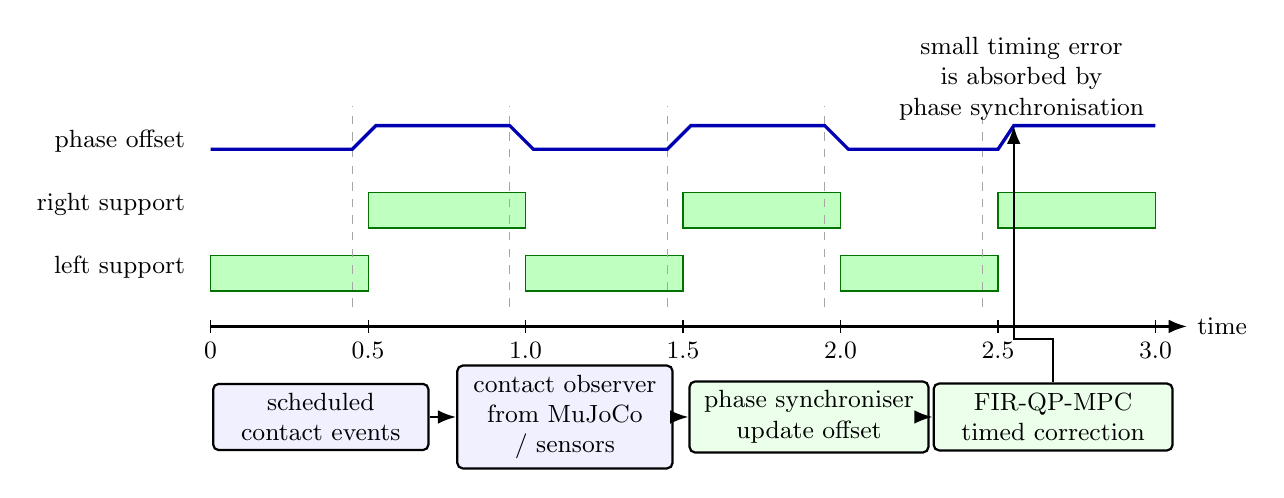
\begin{tikzpicture}[font=\small, >=Latex]
\tikzset{labelbox/.style={draw, rounded corners=2pt, thick, align=center, text width=2.5cm, minimum height=0.75cm, fill=blue!6},
proc/.style={draw, rounded corners=2pt, thick, align=center, text width=2.8cm, minimum height=0.85cm, fill=green!8}}
\draw[->, thick] (0,0) -- (12.4,0) node[right] {time};
\foreach \x/\lab in {0/0,2/0.5,4/1.0,6/1.5,8/2.0,10/2.5,12/3.0} {
  \draw (\x,0.08) -- (\x,-0.08) node[below] {\lab};
}
\node[anchor=east] at (-0.2,0.75) {left support};
\node[anchor=east] at (-0.2,1.55) {right support};
\node[anchor=east] at (-0.2,2.35) {phase offset};
\foreach \x in {0,4,8} {\fill[green!25, draw=green!45!black] (\x,0.45) rectangle +(2.0,0.45);}
\foreach \x in {2,6,10} {\fill[green!25, draw=green!45!black] (\x,1.25) rectangle +(2.0,0.45);}
\foreach \x in {1.8,3.8,5.8,7.8,9.8} {\draw[dashed, gray!70] (\x,0.25) -- (\x,2.8);}
\draw[blue!70!black, very thick] (0,2.25) -- (1.8,2.25) -- (2.1,2.55) -- (3.8,2.55) -- (4.1,2.25) -- (5.8,2.25) -- (6.1,2.55) -- (7.8,2.55) -- (8.1,2.25) -- (10.0,2.25) -- (10.2,2.55) -- (12,2.55);
\node[align=center, text width=3.2cm] at (10.3,3.15) {small timing error\\is absorbed by\\phase synchronisation};
\node[labelbox] (sched) at (1.4,-1.15) {scheduled\\contact events};
\node[labelbox] (obs) at (4.5,-1.15) {contact observer\\from MuJoCo / sensors};
\node[proc] (sync) at (7.6,-1.15) {phase synchroniser\\update offset};
\node[proc] (mpc) at (10.7,-1.15) {FIR-QP-MPC\\timed correction};
\draw[->, thick] (sched) -- (obs);
\draw[->, thick] (obs) -- (sync);
\draw[->, thick] (sync) -- (mpc);
\draw[->, thick] (mpc.north) -- ++(0,0.55) -| (10.2,2.55);
\end{tikzpicture}%
}
\caption{Contact-phase synchronisation concept used by the C2 controller. Observed contact events are compared with the scheduled support sequence, and the resulting phase offset is used to time the FIR-QP-MPC correction.}
\label{fig:c2_contact_phase_synchronisation_timeline}
\end{figure}
 
The final current C1 controller is a fixed-time-phase, reference-aligned empirical FIR-QP-MPC correction layer. It is best presented as a correction layer around the validated C0 replay baseline rather than as a replacement for the offline FDDP planner. It uses the C0 MuJoCo baseline pitch as the reference, the identified FIR model for correction response, a local AR model for natural disturbance decay, and a box-constrained projected-gradient QP solver.
 
The QP controls the scalar correction variable $\alpha$, which is mapped to six joint-position corrections through $G$. The command sent to the actuator proxy remains
\begin{equation}
    \mathbf{q}_{\mathrm{cmd}} = \mathbf{q}_{\mathrm{ref}} + G\alpha.
\end{equation}
The controller updates at \SI{50}{\hertz}, uses a 12-step prediction horizon of \SI{0.24}{\second}, and enforces the constraints summarised in Table~\ref{tab:qp_constraints}.
 
\begin{table}[htbp]
\centering
\caption{Main C1 FIR-QP-MPC constraints.}
\label{tab:qp_constraints}
\begin{tabular}{@{}ll@{}}
\toprule
Constraint & Value \\
\midrule
Correction bound & $|\alpha| \leq \ang{5}$ \\
Slew bound & $\ang{1}$ per \SI{20}{\milli\second} update \\
Maximum accepted joint correction & $\ang{1.5}$ \\
\bottomrule
\end{tabular}
\end{table}
 
% ==================================================================
\chapter{Experimental Validation and Results}\label{ch:experiments}
% ==================================================================
 
This chapter presents the experimental evidence. Section~\ref{sec:validation_scenario} defines the validation scenario and metrics. Section~\ref{sec:c0_c1_comparison} reports the C0 versus C1 comparison. Section~\ref{sec:c2_phase_sync} presents the C2 contact-phase synchronisation results and the scripted alternating-step preview. Section~\ref{sec:detailed_evidence} reports the detailed E1--E6 evidence items, including FDDP convergence, FIR holdout validation, contact-timing comparison, and online timing. Section~\ref{sec:stage9_robustness} presents the Stage~9 software robustness matrix.
 
% ------------------------------------------------------------------
\section{Validation Scenario and Metrics}\label{sec:validation_scenario}
% ------------------------------------------------------------------
 
The current validation uses a controlled synthetic disturbance applied at $t=\SI{0.4}{\second}$: a root-pitch disturbance of \ang{2} and a root pitch-rate disturbance of \SI{0.25}{\radian\per\second}. The same disturbance is applied to both forward and backward CoM-shift cases.
 
The primary evaluation metrics are: integrated absolute pitch error (IAPE, in degree-seconds), settling time to $\pm\ang{0.5}$ (in seconds), maximum joint correction magnitude (in degrees), minimum contact count during the trial, and median QP solve time (in milliseconds). IAPE is the main comparison metric because it captures the cumulative deviation over the full trial rather than only the peak error.
 
% ------------------------------------------------------------------
\section{C0 versus C1 Comparison}\label{sec:c0_c1_comparison}
% ------------------------------------------------------------------
 
Table~\ref{tab:c0_c1_results} summarises the C0 and C1 comparison. The improvement mainly occurs during the recovery phase; the initial pitch peak is essentially unchanged and should not be claimed as reduced.
 
\begin{table}[htbp]
\centering
\caption{Current C0 versus C1 validation results under the controlled pitch disturbance.}
\label{tab:c0_c1_results}
\begin{tabular}{@{}llll@{}}
\toprule
Metric & Direction & C0 & C1 balanced \\
\midrule
Integrated absolute pitch error & Forward & 0.2710 deg s & 0.2474 deg s \\
Improvement & Forward & -- & 8.7\% \\
Settling time to $\pm\ang{0.5}$ & Forward & \SI{0.248}{\second} & \SI{0.166}{\second} \\
Maximum joint correction & Forward & -- & approximately \ang{0.71} \\
Minimum contact count & Forward & -- & 4 \\
Median QP solve time & Forward & -- & \SI{0.60}{\milli\second} \\
\midrule
Integrated absolute pitch error & Backward & 0.2681 deg s & 0.2295 deg s \\
Improvement & Backward & -- & 14.4\% \\
Settling time to $\pm\ang{0.5}$ & Backward & \SI{0.246}{\second} & \SI{0.166}{\second} \\
Maximum joint correction & Backward & -- & approximately \ang{0.67} \\
Minimum contact count & Backward & -- & 4 \\
Median QP solve time & Backward & -- & \SI{0.64}{\milli\second} \\
\bottomrule
\end{tabular}
\end{table}
 
% ------------------------------------------------------------------
\section{C2 Contact-Phase Synchronisation and Scripted Alternating-Step Preview}\label{sec:c2_phase_sync}
% ------------------------------------------------------------------
 
This section presents the figures that provide the main visual evidence for the C2 controller and the scripted alternating-step preview. These figures replace the placeholder result figures from earlier drafts.
 
\begin{figure}[htbp]
\centering
\includegraphics[width=0.92\textwidth]{c2_phase_sync_forward_pitch_comparison.png}
\caption{Forward C2 contact-phase-synchronised FIR-QP-MPC pitch response compared with the nominal replay baseline.}
\label{fig:c2_phase_sync_forward_pitch_comparison}
\end{figure}
 
\begin{figure}[htbp]
\centering
\includegraphics[width=0.92\textwidth]{c2_phase_sync_backward_pitch_comparison.png}
\caption{Backward C2 contact-phase-synchronised FIR-QP-MPC pitch response compared with the nominal replay baseline.}
\label{fig:c2_phase_sync_backward_pitch_comparison}
\end{figure}
 
\begin{figure}[htbp]
\centering
\includegraphics[width=0.92\textwidth]{c2_contact_switching_demo_phase_offset.png}
\caption{C2 contact-switching demonstration showing the controller phase offset used to align correction timing with the support-contact schedule.}
\label{fig:c2_contact_switching_phase_offset}
\end{figure}
 
\begin{figure}[htbp]
\centering
\includegraphics[width=0.92\textwidth]{c2_contact_switching_demo_contacts.png}
\caption{C2 contact-switching demonstration showing scheduled and observed support-contact changes during the preview.}
\label{fig:c2_contact_switching_contacts}
\end{figure}
 
\begin{figure}[htbp]
\centering
\includegraphics[width=0.92\textwidth]{stage8_scripted_alternating_step_contacts.png}
\caption{Stage~8 scripted alternating-step preview contact schedule and measured contact state.}
\label{fig:stage8_scripted_alternating_step_contacts}
\end{figure}
 
\begin{figure}[htbp]
\centering
\includegraphics[width=0.92\textwidth]{stage8_scripted_alternating_step_phase_offset.png}
\caption{Stage~8 scripted alternating-step preview phase-offset evolution used for contact-event synchronisation.}
\label{fig:stage8_scripted_alternating_step_phase_offset}
\end{figure}
 
\begin{figure}[htbp]
\centering
\includegraphics[width=0.92\textwidth]{stage8_scripted_alternating_step_body.png}
\caption{Stage~8 scripted alternating-step preview body-height and torso-pitch response.}
\label{fig:stage8_scripted_alternating_step_body}
\end{figure}
 
% ------------------------------------------------------------------
\section{Detailed Validation Evidence (E1--E6)}\label{sec:detailed_evidence}
% ------------------------------------------------------------------
 
\subsection{E1: FDDP Convergence and Feasibility}
The double-support FDDP continuation was evaluated over twelve CoM-shift amplitudes in each direction. A solver callback retained total cost, maximum and RMS shooting gap, stopping criterion, primal regularisation, step length, and iteration wall time. All 24 continuation stages passed the configured convergence and feasibility gates, producing 48 iteration records. The final maximum shooting gap was zero in both directions; requested shifts of $\pm\SI{6.000}{\milli\metre}$ produced $\pm\SI{6.038}{\milli\metre}$ in the optimised reference.
 
\begin{figure}[htbp]
\centering
\includegraphics[width=0.92\textwidth]{e1_fddp_cost_and_gap.png}
\caption{E1: iteration-level FDDP total cost and maximum shooting gap.}
\label{fig:e1_fddp_cost_gap}
\end{figure}
 
\begin{figure}[htbp]
\centering
\includegraphics[width=0.92\textwidth]{e1_fddp_iteration_time.png}
\caption{E1: FDDP iteration wall time across the forward and backward continuation solves.}
\label{fig:e1_fddp_time}
\end{figure}

\input{fddp_swing_step_evidence_update}
 
\subsection{E2--E3: C0 Replay and C1 Correction (referenced from Sections~\ref{sec:c0_baseline} and~\ref{sec:online_correction})}
The C0 replay results are reported in Table~\ref{tab:c0_metrics} (Section~\ref{sec:c0_baseline}). The C0 versus C1 comparison is reported in Table~\ref{tab:c0_c1_results} (Section~\ref{sec:c0_c1_comparison}).
 
\subsection{E4: FIR Sign-Held-Out Validation}
The FIR model was evaluated independently of the controller. For each direction, a kernel identified from one calibration-pulse polarity predicted the opposite polarity. The four held-out multi-step RMSE values were between $0.0216$ and $0.0224$ degrees, with NRMSE between $0.0546$ and $0.0579$. The estimated delay was \SI{20}{\milli\second}. This is a sign-held-out test, not multi-trial statistical generalisation, because one positive and one negative calibration pulse are currently available per direction.
 
\begin{figure}[htbp]
\centering
\includegraphics[width=0.92\textwidth]{e4_fir_holdout_measured_vs_predicted.png}
\caption{E4: FIR measured-versus-predicted response on a pulse not used to identify the corresponding kernel.}
\label{fig:e4_fir_holdout}
\end{figure}
 
\subsection{E5: C1 versus C2 Contact-Timing Mismatch Comparison}
Fixed-phase C1 and phase-synchronised C2 were compared using the same scripted event sequence under early touchdown, late touchdown, sensor delay, and short contact-loss injections. C1 preserves the planned clock and therefore has zero phase correction. C2 matched all scheduled events in the four software-injected cases and retained a maximum phase correction of \SI{20}{\milli\second}. This is event-layer software validation; it is not a terrain-dynamics or full walking experiment.
 
\begin{figure}[htbp]
\centering
\includegraphics[width=0.92\textwidth]{e5_c1_c2_phase_error_comparison.png}
\caption{E5: fixed-phase C1 and event-synchronised C2 under controlled contact-timing mismatches.}
\label{fig:e5_c1_c2_phase}
\end{figure}
 
\subsection{E6: Online Timing and Available Safety Evidence}
All C1/C2 tests use a \SI{20}{\milli\second} control period. Across four forward/backward runs, the QP P95 solve time ranged from \SI{0.754}{\milli\second} to \SI{1.082}{\milli\second}; the maximum observed solve time was \SI{1.508}{\milli\second}. No QP update missed the \SI{20}{\milli\second} deadline.
 
\begin{table}[htbp]
\centering
\caption{E6 online QP timing evidence.}
\label{tab:e6_timing}
\begin{tabular}{@{}lrrrr@{}}
\toprule
Run & P50 (us) & P95 (us) & Max (us) & Deadline misses \\
\midrule
C1 forward & 679.828 & 809.436 & 1507.705 & 0 \\
C1 backward & 702.078 & 1082.478 & 1385.772 & 0 \\
C2 forward & 640.680 & 772.651 & 932.861 & 0 \\
C2 backward & 658.416 & 753.813 & 899.218 & 0 \\
\bottomrule
\end{tabular}
\end{table}
 
The current logs contain applied corrections but no explicit position-clip, speed-clip, increment-clip, or fallback counters. These quantities are therefore unavailable, not assumed to be zero.
 
\begin{figure}[htbp]
\centering
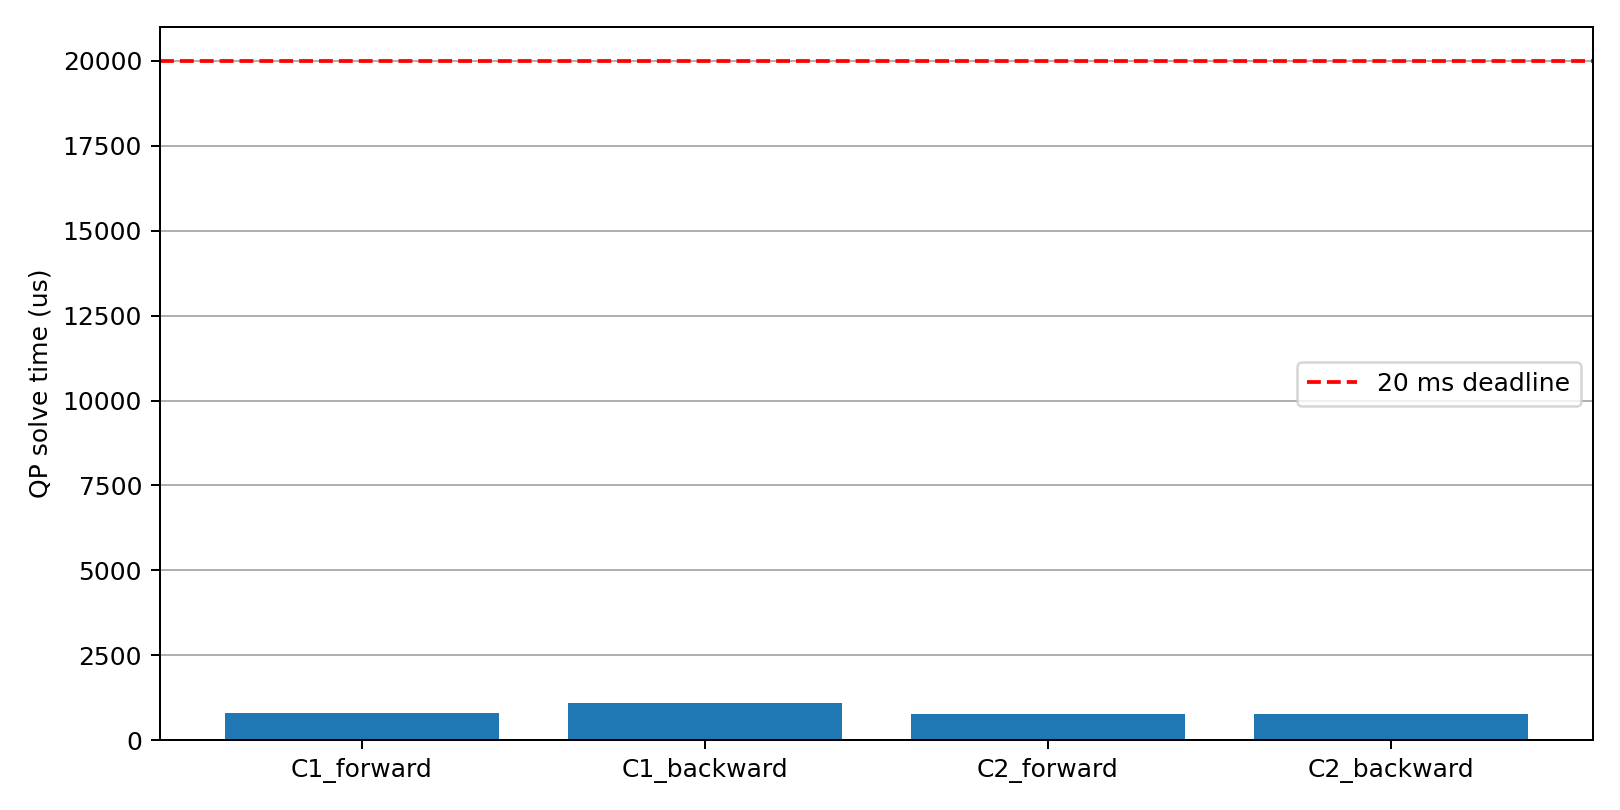
\includegraphics[width=0.82\textwidth]{e6_controller_timing_distribution.png}
\caption{E6: QP P95 solve-time evidence relative to the controller deadline.}
\label{fig:e6_timing}
\end{figure}
 
% ------------------------------------------------------------------
\section{Stage 9 Software Robustness Matrix}\label{sec:stage9_robustness}
% ------------------------------------------------------------------
 
To strengthen the stability and robustness evidence, a Stage~9 software-only robustness matrix was added around the current scripted C2 alternating-step preview. The test matrix extends the previous short Stage~8 contact-transition preview to longer durations and additional stress conditions: long-duration operation, friction variation, slope-equivalent loading, small raised toe-step contacts, and external push pulses.
 
The matrix should be interpreted carefully. It validates the current software stack and MuJoCo contact-event plumbing under scripted periodic stepping. It is not a newly solved full FDDP walking trajectory, and it is not hardware walking validation. It is nevertheless useful because it turns the robustness claim from an untested statement into a measured simulation envelope.
 
\begin{figure}[htbp]
\centering
\resizebox{\textwidth}{!}{%
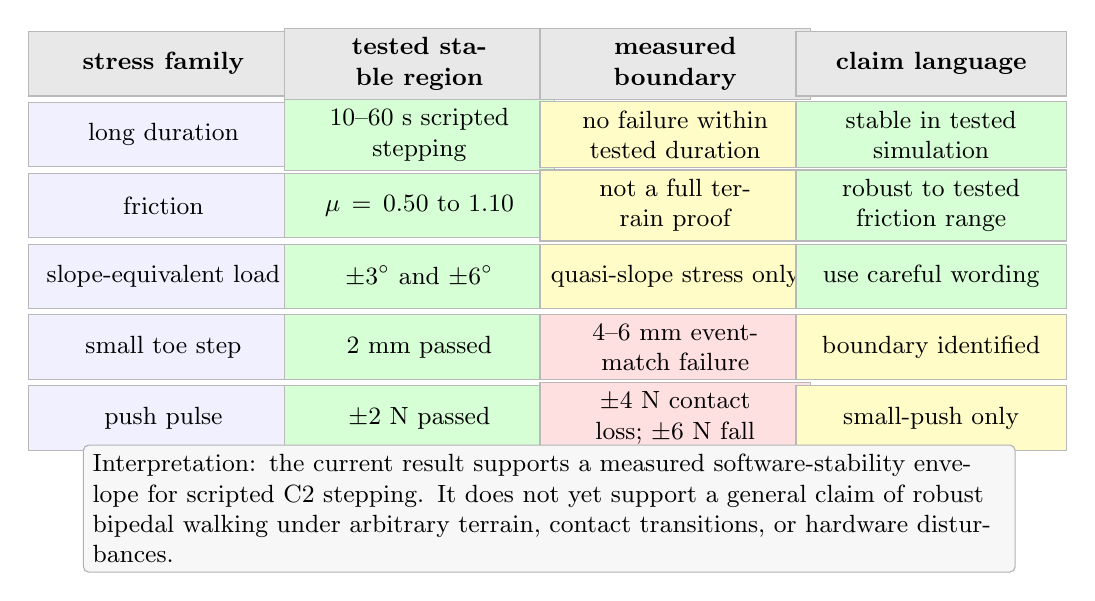
\begin{tikzpicture}[font=\small]
\tikzset{cell/.style={draw=gray!55, align=center, minimum height=0.82cm, text width=3.2cm},
head/.style={cell, fill=gray!18, font=\bfseries\small},
pass/.style={cell, fill=green!16},
bound/.style={cell, fill=yellow!22},
fail/.style={cell, fill=red!12},
neutral/.style={cell, fill=blue!6}}
\node[head] at (0,0) {stress family};
\node[head] at (3.25,0) {tested stable region};
\node[head] at (6.5,0) {measured boundary};
\node[head] at (9.75,0) {claim language};
\node[neutral] at (0,-0.9) {long duration};
\node[pass] at (3.25,-0.9) {10--60 s scripted stepping};
\node[bound] at (6.5,-0.9) {no failure within tested duration};
\node[pass] at (9.75,-0.9) {stable in tested simulation};
\node[neutral] at (0,-1.8) {friction};
\node[pass] at (3.25,-1.8) {$\mu=0.50$ to $1.10$};
\node[bound] at (6.5,-1.8) {not a full terrain proof};
\node[pass] at (9.75,-1.8) {robust to tested friction range};
\node[neutral] at (0,-2.7) {slope-equivalent load};
\node[pass] at (3.25,-2.7) {$\pm 3^{\circ}$ and $\pm 6^{\circ}$};
\node[bound] at (6.5,-2.7) {quasi-slope stress only};
\node[pass] at (9.75,-2.7) {use careful wording};
\node[neutral] at (0,-3.6) {small toe step};
\node[pass] at (3.25,-3.6) {2 mm passed};
\node[fail] at (6.5,-3.6) {4--6 mm event-match failure};
\node[bound] at (9.75,-3.6) {boundary identified};
\node[neutral] at (0,-4.5) {push pulse};
\node[pass] at (3.25,-4.5) {$\pm 2$ N passed};
\node[fail] at (6.5,-4.5) {$\pm 4$ N contact loss; $\pm 6$ N fall};
\node[bound] at (9.75,-4.5) {small-push only};
\node[draw=gray!60, rounded corners=2pt, align=left, text width=11.6cm, fill=gray!6] at (4.9,-5.65) {Interpretation: the current result supports a measured software-stability envelope for scripted C2 stepping. It does not yet support a general claim of robust bipedal walking under arbitrary terrain, contact transitions, or hardware disturbances.};
\end{tikzpicture}%
}
\caption{Stage~9 robustness envelope and claim boundary. Green cells identify stable tested regions, yellow cells mark interpretation limits, and red cells mark measured failure boundaries.}
\label{fig:stage9_robustness_envelope_claim_boundary}
\end{figure}
 
\begin{table}[htbp]
\centering
\caption{Stage~9 scripted C2 software robustness matrix.}
\label{tab:stage9_robustness_matrix_20260708}
\scriptsize
\begin{tabular}{@{}p{0.14\textwidth}p{0.17\textwidth}p{0.08\textwidth}p{0.22\textwidth}p{0.22\textwidth}@{}}
\toprule
Stress family & Tested range & Pass/total & \shortstack{Strongest\\passing case} & \shortstack{First failing\\boundary} \\
\midrule
Long duration & \SI{10}{\second}, \SI{30}{\second}, \SI{60}{\second} & 3/3 & \SI{60}{\second}, 119/120 events matched & none tested \\
Friction & $\mu=0.50$ to $\mu=1.10$ & 4/4 & $\mu=0.50$, peak pitch \SI{0.82}{\degree} & none tested \\
Slope-equivalent load & $\pm\SI{3}{\degree}$, $\pm\SI{6}{\degree}$ & 4/4 & $-\SI{6}{\degree}$, peak pitch \SI{1.55}{\degree} & none tested \\
Small toe step & \SI{2}{\milli\metre}, \SI{4}{\milli\metre}, \SI{6}{\milli\metre} & 1/3 & \SI{2}{\milli\metre}, 17/20 events matched & \SI{4}{\milli\metre} event-match failure \\
Push pulse & $\pm\SI{2}{\newton}$, $\pm\SI{4}{\newton}$, $\pm\SI{6}{\newton}$ & 2/6 & $\pm\SI{2}{\newton}$ no fall & $\pm\SI{4}{\newton}$ contact loss; $\pm\SI{6}{\newton}$ fall \\
\midrule
Total & 20 scenarios & 14/20 & -- & -- \\
\bottomrule
\end{tabular}
\end{table}
 
The aggregate pass/fail result and peak-pitch envelope are visualised in Figures~\ref{fig:stage9_robustness_pass_fail} and~\ref{fig:stage9_robustness_peak_pitch}.
 
\begin{figure}[htbp]
\centering
\includegraphics[width=0.92\textwidth]{stage9_scripted_robustness_matrix_pass_fail.png}
\caption{Stage~9 software robustness matrix pass/fail outcome across duration, friction, slope-equivalent loading, small-step, and push-pulse scenarios.}
\label{fig:stage9_robustness_pass_fail}
\end{figure}
 
\begin{figure}[htbp]
\centering
\includegraphics[width=0.92\textwidth]{stage9_scripted_robustness_matrix_pitch.png}
\caption{Peak absolute torso pitch across the Stage~9 scripted robustness matrix.}
\label{fig:stage9_robustness_peak_pitch}
\end{figure}
 
The most stable part of the envelope is long-duration scripted stepping on flat terrain. The \SI{60}{\second} case matched 119/120 scheduled contact events, kept peak pitch below \SI{0.81}{\degree}, and did not trigger a fall. Friction variation from $\mu=0.50$ to $\mu=1.10$ and slope-equivalent loading up to $\pm\SI{6}{\degree}$ also passed the current acceptance criteria.
 
The matrix also identifies the current robustness boundary. A \SI{2}{\milli\metre} raised toe step passed, but \SI{4}{\milli\metre} and \SI{6}{\milli\metre} steps failed the event-matching/contact robustness criteria. Push pulses of $\pm\SI{2}{\newton}$ passed, while $\pm\SI{4}{\newton}$ caused transient support contact loss without a fall, and $\pm\SI{6}{\newton}$ crossed the \SI{30}{\degree} pitch fall threshold after approximately \SI{2.2}{\second}. These failures should be reported as measured limits of the current scripted controller rather than hidden or relaxed.
 
The resulting conclusion from the Stage~9 matrix is therefore:
\begin{quote}
The current software stack is stable under the tested long-duration, friction, slope-equivalent, low-step-height, and small-push simulation conditions. The current scripted controller is not robust to larger toe-step perturbations or large push pulses. Full FDDP walking-gait validation and hardware walking experiments remain required before claiming general robust biped locomotion.
\end{quote}
 
The supporting files are:
\begin{itemize}
    \item \path{results/logs/stage9_scripted_robustness_matrix_summary.yaml}
    \item \path{results/logs/stage9_scripted_robustness_matrix_table.csv}
    \item \path{results/figures/stage9_scripted_robustness_matrix_pass_fail.png}
    \item \path{results/figures/stage9_scripted_robustness_matrix_pitch.png}
\end{itemize}
 
% ------------------------------------------------------------------
\section{Evidence Traceability Matrix}\label{sec:evidence_traceability}
% ------------------------------------------------------------------
 
Table~\ref{tab:evidence_traceability} provides a working traceability matrix mapping each claim type to the supporting artifact, its current status, and its evidential boundary.
 
\begin{table}[htbp]
\centering
\caption{Working evidence traceability matrix for the current simulation results.}
\label{tab:evidence_traceability}
\begin{tabular}{@{}p{0.24\linewidth}p{0.28\linewidth}p{0.18\linewidth}p{0.22\linewidth}@{}}
\toprule
Claim type & Required artifact & Current status & Boundary \\
\midrule
FDDP planning progresses from double support through single/two-step contact switches & FDDP logs, support/landing/clearance gates, replay artifacts, and contact-feasibility report & Layered evidence & Single/two-step accepted; ten-step final nominal withheld after friction/CoP failure \\
C0 replay remains stable under actuator-aware proxy & MuJoCo replay logs, joint RMSE, torso pitch, torso height, contact count & Ready for current cases & Simulation proxy, not measured hardware \\
C1 reduces integrated pitch error & C0/C1 paired sweep CSV and plot & Ready for controlled disturbance & Recovery phase only; not initial peak reduction \\
C1 reduces settling time & C0/C1 settling-time table and pitch-error plot & Ready for controlled disturbance & Threshold-dependent metric \\
QP computation is below 1 ms in Python simulation & Timing log from C1 sweep & Ready for current machine/setup & Not hard real-time hardware proof \\
Controller maintains the declared contact minimum in tested cases & Contact-count and per-foot event logs & Ready for stated cases & Not continuous gait or rough-terrain validation \\
\bottomrule
\end{tabular}
\end{table}
 
% ==================================================================
\chapter{Discussion}\label{ch:discussion}
% ==================================================================
 
This chapter interprets the results presented in Chapter~\ref{ch:experiments}, discusses their limitations, and examines threats to validity. Each section addresses a distinct finding cluster.
 
% ------------------------------------------------------------------
\section{Interpretation of FDDP Convergence and the Derivative Audit (E1)}
% ------------------------------------------------------------------
 
The E1 continuation sweep demonstrates that the offline FDDP planner reliably converges for double-support CoM shifts across the tested $\pm\SI{6}{\milli\metre}$ range. All 24 continuation stages passed their convergence and feasibility gates, and the final shooting gap reached zero in both directions. The small discrepancy between the requested shift ($\pm\SI{6.000}{\milli\metre}$) and the optimised reference ($\pm\SI{6.038}{\milli\metre}$) is attributable to the soft penalty formulation of the CoM tracking cost rather than a solver failure: the optimiser trades a small tracking error against other cost terms such as state regularisation and joint-limit avoidance.
 
The derivative-consistency audit reveals a practical point that is under-reported in the FDDP literature: the default damping settings that work for well-conditioned models may produce unacceptably large derivative errors for small, stiff, contact-constrained models. The selection of $\texttt{JMinvJt\_damping}=10^{-8}$ was driven by the observation that a zero-damping configuration---while it did not crash the solver---produced $F_x$ relative errors that would undermine the quadratic convergence assumptions of DDP. Researchers applying FDDP to small biped models should be aware that damping tuning and derivative auditing are necessary preconditions for reliable trajectory optimisation, not optional checks.

% ------------------------------------------------------------------
\section{Interpretation of Incremental Swing-Step and Multi-Step FDDP Evidence}
% ------------------------------------------------------------------

The new swing-step results extend the planner beyond double support, but the evidence is deliberately layered. The independent left- and right-swing problems achieve zero shooting gap and pass support, landing, clearance, joint-margin, and forward-CoM gates, yet both terminate at the 500-iteration budget with a first-order stopping criterion near $10^{-3}$. They demonstrate specified physical feasibility and replayability, not first-order convergence. The two-step alternating problem is stronger convergence evidence: it reaches a stopping criterion of $2.84\times10^{-8}$ and passes the declared trajectory gates before position-command replay.

The periodic-cycle and 4/6/10-step continuation results show that longer FDDP planning is numerically possible. However, the ten-step candidate fails a separate planar support-resultant audit at 75 of 1000 support nodes, with maximum friction utilisation 2.165 against a 0.90 gate and minimum CoP margin $-416.6$~mm against a required 2~mm margin. This negative result is important: zero shooting gap and accurate foot placement do not guarantee physically acceptable contact wrenches. Withholding the final nominal and its replay is therefore part of the validation method, not an unfinished reporting step.
 
% ------------------------------------------------------------------
\section{Interpretation of C0 Replay and Actuator/Model Mismatch}
% ------------------------------------------------------------------
 
The C0 replay results establish that the FDDP nominal trajectory is stable under actuator-aware replay without online correction for the tested double-support CoM-shift case. The achieved MuJoCo CoM displacement ($\pm\SI{6.53}{\milli\metre}$) exceeds the FDDP target ($\pm\SI{6.00}{\milli\metre}$) by approximately 9\%, and the ankle joint RMSE ($\ang{0.398}$) is larger than the hip and knee RMSE values. Both observations are consistent with the actuator proxy model: the ankle joints experience the largest load during double support, so the first-order lag and speed saturation have the greatest effect there.
 
This mismatch is not a failure of the FDDP planner---the planner optimises in torque space under ideal actuator assumptions---but rather a consequence of the position-controlled, bandwidth-limited actuation concept. It is precisely this mismatch that motivates the online correction layer: if the C0 replay were already perfect, C1 would have nothing to improve.
 
% ------------------------------------------------------------------
\section{Interpretation of C0 versus C1 Recovery Improvement}
% ------------------------------------------------------------------
 
The C1 FIR-QP-MPC controller reduces integrated absolute pitch error by 8.7\% (forward) and 14.4\% (backward) relative to C0, and reduces settling time from approximately \SI{0.247}{\second} to \SI{0.166}{\second} in both directions. Importantly, the initial pitch peak is essentially unchanged between C0 and C1. This pattern---unchanged peak, improved recovery---is consistent with the FIR model structure. The FIR impulse response has its peak magnitude at a delay of \SI{0.20}{\second}, so the controller cannot counteract the initial disturbance before the correction propagates through the actuator dynamics. Once the correction takes effect, however, the controller accelerates the return to the reference pitch.
 
The asymmetry in improvement (8.7\% forward versus 14.4\% backward) may reflect small asymmetries in the MuJoCo model or in the calibration condition, but the difference is small enough that both directions show a consistent qualitative benefit. Further calibration trials would be needed to determine whether the asymmetry is reproducible or a single-trial artefact.
 
% ------------------------------------------------------------------
\section{Interpretation of the FIR Sign-Held-Out Validation (E4)}
% ------------------------------------------------------------------
 
The E4 results provide the strongest independent evidence that the FIR model captures genuine pitch dynamics rather than overfitting to a single calibration pulse. When a kernel identified from a positive calibration pulse is used to predict the response to a negative pulse (or vice versa), the held-out RMSE remains below \ang{0.023} and the NRMSE below 0.058. This is strong evidence given that the kernel is identified from a single trial and tested on the opposite polarity without retuning.
 
The limitation is equally important: this is a sign-held-out test with one trial of each polarity per direction. It demonstrates that the FIR parameters generalise across the sign of the correction, but it does not demonstrate generalisation across a wider range of disturbance amplitudes, joint configurations, or contact modes. The FIR model should therefore be treated as a locally valid empirical representation, not a globally identified actuator model.
 
% ------------------------------------------------------------------
\section{Interpretation of C2 Contact-Phase Synchronisation (E5)}
% ------------------------------------------------------------------
 
The C1 versus C2 comparison demonstrates that contact-event phase synchronisation correctly aligns the correction reference under software-injected timing mismatches: early touchdown, late touchdown, sensor delay, and short contact loss. C2 matched all scheduled events in the four tested cases, while C1---which uses the planned clock without correction---accumulated a phase offset that would degrade correction timing in a longer trial.
 
This result validates the event-layer plumbing of the C2 controller: the scheduled contact sequence, the MuJoCo contact observer, and the phase-offset computation are functioning correctly as a software pipeline. What this result does not validate is that the synchroniser would work under the more complex, noisy, and unpredictable contact dynamics of actual terrain. The injected mismatches are deterministic and known to the test harness; real terrain produces stochastic contact timing variations that may interact with the synchroniser in ways not captured by the current test set.
 
% ------------------------------------------------------------------
\section{Interpretation of Online Timing (E6)}
% ------------------------------------------------------------------
 
The QP solve-time evidence is unequivocal: across all four C1/C2 configurations, the P95 solve time is at most \SI{1.082}{\milli\second}, well below the \SI{20}{\milli\second} control period. No deadline was missed. This confirms that the scalar-QP formulation with a 12-step FIR prediction horizon is computationally viable in the current Python implementation.
 
However, this timing evidence should not be interpreted as proof of hard real-time capability. The measurements were taken on a single machine under a single software configuration; they do not include worst-case execution time analysis, operating-system scheduling guarantees, or the additional computational load of sensor processing and communication that would accompany hardware deployment. The timing evidence supports the claim that the QP is not the computational bottleneck; it does not support the claim that the full control loop meets hard real-time constraints on embedded hardware.
 
% ------------------------------------------------------------------
\section{Interpretation of the Stage~9 Robustness Envelope}
% ------------------------------------------------------------------
 
The Stage~9 robustness matrix provides the most comprehensive evidence of the current software stack's stability boundary. The results can be read as a contour map: the controller is stable in the interior (long duration, moderate friction variation, slope-equivalent loading, small push pulses) and fails at the edges (larger toe steps, larger push pulses). This is exactly the pattern expected of a controller that was designed for disturbance recovery around a nominal trajectory rather than for general gait robustness.
 
The failure modes are informative. The toe-step failures at \SI{4}{\milli\metre} and \SI{6}{\milli\metre} are event-match failures: the MuJoCo contact observer cannot reliably detect the early or late touchdown caused by the raised step, so the phase synchroniser receives incorrect event timing. This is a sensor/observer limitation, not a control instability per se. The push-pulse failures at $\pm\SI{4}{\newton}$ and $\pm\SI{6}{\newton}$ are more fundamental: the joint-position correction authority of $\pm\ang{1.5}$ per joint is insufficient to counteract the induced pitch momentum within the available horizon. These are genuine control-authority limits, and they define a measurable boundary of the current architecture.
 
% ------------------------------------------------------------------
\section{Aggregate Limitations}
% ------------------------------------------------------------------
 
Table~\ref{tab:validation_roadmap} consolidates the validated claims, near-term tasks, and explicit limitations discussed throughout this chapter.
 
\begin{table}[htbp]
\centering
\caption{Validation roadmap and claim boundary.}
\label{tab:validation_roadmap}
\begin{tabular}{@{}p{0.28\linewidth}p{0.28\linewidth}p{0.34\linewidth}@{}}
\toprule
Validation item & Current status & Thesis treatment \\
\midrule
Double-support nominal CoM shift & Implemented and simulated & E1 convergence result \\
Independent left/right FDDP swing steps & Physical gates and position-command replay passed & Not first-order convergence success \\
Two-step alternating FDDP reference & Converged, gated, replayed & Fixed two-step evidence; not continuous gait \\
Ten-step FDDP planning candidate & Planning gates passed; friction/CoP gate failed & Final nominal and replay withheld \\
Actuator-aware C0 replay & Implemented with assumed proxy & Main baseline \\
Fixed-phase FIR-QP-MPC C1 & Implemented and simulated & Main correction result \\
Independent FIR sign-held-out validation & Implemented & Four polarity-held-out splits; limited trial count \\
Contact-event phase synchronisation C2 & Implemented in simulation & Injected mismatch evidence plus two-step natural-event retiming; no universal recovery gain \\
Scripted C2 robustness envelope & Implemented (20 scenarios) & Measured software stability boundary \\
Actuator-parameter sensitivity & Not yet complete & Future work or optional extension \\
Sensor noise and timing jitter & Not yet included & Limitation \\
Hardware validation & Not completed & Explicit limitation \\
Continuous multi-step FDDP replay & Not completed & Ten-step contact gate currently fails \\
\bottomrule
\end{tabular}
\end{table}
 
The principal limitations are as follows. First, validation is simulation-only: the MuJoCo contact model, the rigid-body dynamics, and the actuator proxy are approximations whose fidelity to physical hardware has not been established. Second, the actuator proxy parameters (delay, lag, speed limit) are engineering assumptions, not experimentally identified ST3215 system-identification results. Third, C2 has both deterministic event-injection evidence and a two-step natural-contact demonstration, but the latter matched three of four scheduled events and did not improve the common pitch-disturbance metric over C1; stochastic terrain timing remains unvalidated. Fourth, the FIR sign-held-out result has only one pulse trial of each polarity per direction, which limits the statistical confidence in the FIR model's generalisation. Fifth, sensor noise, IMU drift, encoder noise, timing jitter, and explicit runtime safety counters remain outside the current validated scope. Sixth, the ten-step planning candidate fails the current friction-utilisation and CoP-margin gates, so there is no final continuous multi-step FDDP nominal or replay.
 
% ------------------------------------------------------------------
\section{Threats to Validity}
% ------------------------------------------------------------------
 
\subsection{Internal validity}
The C0/C1 comparison uses the same disturbance, the same trajectory, and the same actuator proxy for both conditions. The only difference is the presence or absence of the FIR-QP-MPC correction layer. This is a well-controlled within-simulation comparison, so the improvement in integrated pitch error and settling time can be attributed to the correction layer rather than to confounding factors. The main internal-validity concern is that the FIR model and the controller were tuned on the same disturbance case (forward direction), which raises the possibility of overfitting. The backward-direction result---which uses the same tuning without modification and shows a similar improvement---partially mitigates this concern, but a multi-disturbance, multi-condition validation would provide stronger evidence.
 
\subsection{External validity}
The external validity of these results is bounded by the simulation domain. The MuJoCo contact model uses a convex approximation that may not capture the stick-slip and micro-deformation behaviour of real foot-ground contact. The actuator proxy is simpler than a real ST3215 servo. The disturbance is a single, deterministic perturbation applied at a known time. These simplifications are appropriate for a simulation-based architectural validation, but they mean that no quantitative prediction about hardware performance can be drawn from the current results.
 
\subsection{Construct validity}
The primary evaluation metric---integrated absolute pitch error---captures cumulative deviation but weights all time periods equally. It does not distinguish between a controller that recovers quickly with a large overshoot and one that recovers slowly without overshoot. Settling time depends on an arbitrary threshold ($\pm\ang{0.5}$). These are standard metrics in the locomotion control literature, and they are reported transparently with their thresholds stated, but readers should be aware that metric choice can influence the apparent magnitude of improvement.
 
\subsection{Reliability}
All results are from single simulation runs. The stochasticity of the MuJoCo solver is minimal at the current timestep, but run-to-run variability has not been quantified. Multi-run statistics would strengthen the reliability of the reported metrics, particularly for the backward-direction C1 improvement, where the 14.4\% figure may vary with initial conditions.
 
% ==================================================================
\chapter{Conclusion and Future Work}\label{ch:conclusion}
% ==================================================================
 
% ------------------------------------------------------------------
\section{Answers to Research Questions}
% ------------------------------------------------------------------
 
This section answers each research question posed in Chapter~\ref{ch:Introduction}, citing the relevant evidence from Chapters~\ref{ch:control_architecture} and~\ref{ch:experiments}.
 
\noindent\textbf{RQ1: How far can offline FDDP progress from double-support CoM shifts to fixed-schedule alternating contact trajectories for the six-DoF planar biped model?}
 
FDDP now progresses through several evidence levels. The E1 continuation sweep reliably converges for $\pm\SI{6}{\milli\metre}$ double-support CoM shifts, with zero final shooting gap and audited derivatives. Independent left- and right-swing DS--SS--DS problems pass their specified physical feasibility gates and position-command replay integrity, although both exhaust the 500-iteration budget and therefore are not first-order convergence successes. The two-step alternating problem converges with solver stop $2.84\times10^{-8}$, zero gap, accepted support/landing/clearance gates, and a completed replay. Periodic and 4/6/10-step planning continuation pass their planning gates, but the ten-step candidate fails the subsequent friction-utilisation and CoP-margin audit. The correct RQ1 answer is therefore positive for double-support, individual swing steps, and a fixed two-step reference, but negative for a final continuous multi-step nominal.
 
\noindent\textbf{RQ2: How does the FDDP nominal trajectory behave under actuator-aware MuJoCo replay without online correction?}
 
The C0 replay (Section~\ref{sec:c0_baseline}, Table~\ref{tab:c0_metrics}) remains stable for the tested forward and backward shifts. The achieved CoM displacement exceeds the FDDP target by approximately 9\%, and ankle joint tracking shows the largest RMSE ($\ang{0.398}$), consistent with the actuator proxy's speed and lag limitations under load. The C0 replay demonstrates that the nominal trajectory is viable but that actuator/model mismatch produces measurable tracking error---this is the gap that the online correction layer is designed to address.
 
\noindent\textbf{RQ3: Can a fast fixed-phase FIR-QP-MPC correction layer improve recovery from controlled pitch disturbances without large joint corrections?}
 
Yes, with quantified boundary conditions. The C1 FIR-QP-MPC controller reduces integrated absolute pitch error by 8.7\% (forward) and 14.4\% (backward), and reduces settling time from approximately \SI{0.247}{\second} to \SI{0.166}{\second} (Table~\ref{tab:c0_c1_results}). The maximum joint correction remains below \ang{0.72}, and the median QP solve time is below \SI{0.65}{\milli\second} (E6, Table~\ref{tab:e6_timing}). The improvement is confined to the recovery phase; the initial pitch peak is essentially unchanged, which is consistent with the FIR model's \SI{0.20}{\second} peak response delay. Support contact is maintained (minimum contact count of 4) in all tested cases.
 
\noindent\textbf{RQ4: Can contact-event phase synchronisation align the correction reference under controlled timing mismatches?}
 
Yes, for software-injected deterministic timing mismatches. The C1/C2 comparison (E5, Section~\ref{sec:detailed_evidence}) shows that C2 matches all scheduled events under early touchdown, late touchdown, sensor delay, and short contact-loss injections, with a maximum phase correction of \SI{20}{\milli\second}. This validates the event-layer plumbing---scheduled contact sequence, MuJoCo contact observer, and phase-offset computation---but does not validate performance under stochastic terrain contact dynamics. That remains a distinct future-work item.
 
% ------------------------------------------------------------------
\section{Thesis Summary}
% ------------------------------------------------------------------
 
This thesis presents a simulation-based control architecture for a low-cost position-controlled six-DoF planar biped. The architecture combines three elements: (i) offline FDDP for contact-consistent nominal trajectory generation, (ii) an actuator-aware C0 replay baseline that isolates nominal trajectory quality from correction benefit, and (iii) a fast FIR-QP-MPC online correction layer that uses an empirically identified pitch-response model and a box-constrained QP solver. The evidence includes double-support FDDP convergence, independent swing-step gates, a converged and replayed two-step reference, a rejected ten-step contact-feasibility candidate, FIR sign-held-out validation, C1/C2 contact-event timing comparisons, QP timing statistics, C0/C1 recovery comparisons, and a Stage~9 scripted robustness envelope. These evidence classes remain explicitly separated so that scripted stepping and planning-only multi-step candidates are not presented as continuous FDDP walking.
 
% ------------------------------------------------------------------
\section{Future Work}
% ------------------------------------------------------------------
 
The most important direction for future work is extending the validation from event-layer simulation to physical contact dynamics and then to hardware. Specific priorities are:
 
\begin{enumerate}[label=\arabic*.]
    \item \textbf{Close the multi-step FDDP contact-feasibility gap.} Single-support swing steps and a converged two-step alternating reference now exist, but the ten-step candidate fails friction-utilisation and CoP-margin gates. Force regularisation, friction/wrench-cone and CoP constraints, verified derivatives, and continuation should be added before any continuous multi-step replay is attempted.
    \item \textbf{Terrain and sensor-delay experiments.} The C2 phase synchroniser should be tested with stochastic contact-timing variation, uneven terrain, and sensor-delay models that approximate real IMU and encoder latency.
    \item \textbf{Actuator-parameter sensitivity.} The actuator proxy parameters (delay, lag, speed limit) should be varied systematically to determine how sensitive the C1/C2 improvement is to these assumptions, and which parameters most affect stability.
    \item \textbf{Sensor-noise tests.} The controller currently receives clean MuJoCo state. Injecting IMU noise, encoder quantisation, and communication dropouts would test whether the FIR-QP-MPC formulation is robust to realistic sensing degradation.
    \item \textbf{Explicit runtime safety counters.} Position-clip, speed-clip, increment-clip, and fallback-mode counters should be added to the logging pipeline so that safety violations can be detected and reported rather than remaining invisible in the logs.
    \item \textbf{Hardware validation pipeline.} A safe, incremental hardware pipeline should be developed, beginning with static joint-command tests, progressing to single-joint dynamic tests, and finally to bench-top biped standing and CoM-shift experiments with IMU and servo encoder feedback. This pipeline should include explicit safety stop conditions and fallback behaviours at each stage.
\end{enumerate}
 
% ══════════════════════════════════════════════════════════════════
% APPENDICES
% ══════════════════════════════════════════════════════════════════
\appendix
 
% ------------------------------------------------------------------
\chapter{Claim-Evidence Matrix}
% ------------------------------------------------------------------
 
\section{Safe Thesis Claims}
 
\begin{longtable}{@{}p{0.28\linewidth}p{0.32\linewidth}p{0.30\linewidth}@{}}
\caption{Safe claims and required evidence before final submission.}\label{tab:claim_evidence_matrix}\\
\toprule
Safe claim & Evidence to cite in Results/Discussion & Language boundary \\
\midrule
\endfirsthead
\toprule
Safe claim & Evidence to cite in Results/Discussion & Language boundary \\
\midrule
\endhead
FDDP generated converged double-support CoM shifts and a converged two-step alternating reference; independent swing steps passed specified physical gates. & E1 records, single/two-step diagnostics, replay artifacts, and exported metadata. & Distinguish first-order convergence from gate passing; do not generalise to continuous gait. \\
The ten-step FDDP planning candidate was rejected by the final contact gate. & Friction/CoP report, failed-node plot, and absence of the final nominal NPZ. & Present as negative evidence; do not claim multi-step replay. \\
The actuator-aware C0 replay remained stable for the tested forward and backward shifts. & C0 replay metrics, contact count, torso height, joint RMSE, achieved CoM displacement. & Say actuator-aware proxy; do not say identified servo dynamics. \\
The C1 FIR-QP-MPC layer reduced integrated pitch tracking error under the controlled disturbance. & Forward/backward C0 versus C1 integrated absolute pitch-error table. & Say recovery-phase improvement; do not claim initial peak reduction. \\
The C1 layer reduced settling time to the chosen threshold. & Settling-time metrics and pitch-error plots. & State the threshold and disturbance condition. \\
The C1 correction required sub-degree maximum joint-position corrections in the tested cases. & Correction magnitude logs for forward/backward cases. & State this is within current simulation and tuning. \\
The QP solve time was below 1 ms in the current Python simulation. & Timing logs from the sweep. & Do not claim hard real-time hardware performance. \\
The C2 phase synchroniser matched scheduled events under software-injected timing mismatches. & C1/C2 phase-error comparison, matched-event ratio. & Say event-layer software validation; not terrain contact dynamics. \\
The Stage~9 scripted C2 controller is stable within the tested envelope. & Robustness matrix pass/fail table, peak-pitch figures. & State tested conditions and measured boundaries explicitly. \\
\bottomrule
\end{longtable}
 
\section{Claims to Avoid}
\begin{itemize}
    \item Do not claim that the controller is hardware validated.
    \item Do not claim that ST3215 servos are torque controlled.
    \item Do not present $\boldsymbol{\tau}_{\mathrm{ref}}$ as a motor command.
    \item Do not generalise the tested C1/two-step result to continuous gait, arbitrary contact phases, or arbitrary disturbances.
    \item Do not claim hard real-time execution from Python simulation timing alone.
    \item Do not claim the initial pitch peak is reduced when the evidence mainly shows improved recovery.
    \item Do not claim terrain-level robustness from event-layer timing-mismatch tests alone.
    \item Do not claim statistical generalisation from the single-trial FIR holdout result.
\end{itemize}
 
% ------------------------------------------------------------------
\chapter{Reproducibility Notes}
% ------------------------------------------------------------------
 
\section{Main Project Files}
\begin{itemize}
    \item \path{model/biped_v1.urdf}
    \item \path{model/biped_planar.xml}
    \item \path{fddp/03m_validate_damped_6d_microshift.py}
    \item \path{fddp/03n_solve_damped_6d_full_continuation.py}
    \item \path{simulation/03o_replay_fddp_com_shift_mujoco.py}
    \item \path{mpc/06_identify_qp_mpc_fir_model.py}
    \item \path{mpc/07_run_reference_aligned_fir_qp_mpc_sweep.py}
\end{itemize}
 
\section{Reporting Checklist}
Each experiment should log contact count, torso height, pitch error, correction magnitude, computation time, controller parameters, actuator-proxy parameters, and trajectory metadata. Results should be saved as CSV, YAML, and figure outputs where possible.
 
% ------------------------------------------------------------------
\chapter{Planned Figure and Table Set}
% ------------------------------------------------------------------
 
Table~\ref{tab:figure_table_plan} lists the figures and tables that should be prepared before expanding the thesis into final prose. Results claims should be written only after the corresponding figure or table exists.
 
\begin{longtable}{@{}p{0.12\linewidth}p{0.38\linewidth}p{0.40\linewidth}@{}}
\caption{Planned figure and table set for the thesis.}\label{tab:figure_table_plan}\\
\toprule
Item & Purpose & Suggested source \\
\midrule
\endfirsthead
\toprule
Item & Purpose & Suggested source \\
\midrule
\endhead
Fig. 1 & Robot model, coordinate convention, and six actuated pitch joints & MuJoCo/URDF render or schematic \\
Fig. 2 & Overall architecture: offline FDDP, C0 replay, FIR identification, C1 QP-MPC & Drawn block diagram \\
Fig. 3 & FDDP CoM-shift nominal trajectories and contact mode & FDDP trajectory export \\
Fig. 4 & Derivative audit summary for damping choice & Audit logs from FDDP validation \\
Fig. 5 & C0 actuator-aware replay tracking and CoM displacement & Replay logs \\
Fig. 6 & Pitch-authority pulse response and FIR fit & FIR identification script output \\
Fig. 7 & C0 versus C1 pitch-error time histories & Final C1 sweep output \\
Fig. 8 & Correction signal, joint correction magnitude, and contact count & Final C1 sweep output \\
Fig. 9 & C2 phase-synchronised forward/backward pitch response & C2 sweep output \\
Fig. 10 & C2 contact-switching phase offset and contact state & C2 sweep output \\
Fig. 11 & Stage~8 scripted alternating-step contacts, phase offset, body response & Stage~8 output \\
Fig. 12 & E1 FDDP cost, gap, and iteration time & FDDP validation output \\
Fig. 13 & E4 FIR sign-held-out measured vs predicted & FIR identification output \\
Fig. 14 & E5 C1 vs C2 phase-error comparison & C1/C2 comparison output \\
Fig. 15 & E6 controller timing distribution & Timing log output \\
Fig. 16 & Stage~9 robustness pass/fail and peak pitch & Stage~9 robustness output \\
Table 1 & Robot geometry and model dimensions & Model files and inspection logs \\
Table 2 & Controller settings and constraints & C1 configuration \\
Table 3 & Forward/backward C0 versus C1 performance metrics & Final C1 sweep output \\
Table 4 & E6 online QP timing evidence & Timing logs \\
Table 5 & Stage~9 robustness matrix & Stage~9 summary YAML/CSV \\
Table 6 & Validation roadmap and limitations & Discussion chapter \\
\bottomrule
\end{longtable}
 
% ══════════════════════════════════════════════════════════════════
% BIBLIOGRAPHY
% ══════════════════════════════════════════════════════════════════
\clearpage
\bibliographystyle{ieeetr}
\bibliography{sample}
 
\end{document}